\documentclass[a0paper,portrait]{baposter}

\usepackage[font=small,labelfont=bf]{caption}
\usepackage{booktabs}
\usepackage{relsize}

\usepackage[colorlinks=true,linkcolor=black,citecolor=black,urlcolor=black]{hyperref}
\usepackage{graphicx}
\usepackage{subcaption}
\usepackage{amsmath}
\usepackage{siunitx}

\graphicspath{{figs/}}

\definecolor{bordercol}{RGB}{40,40,40}
\definecolor{headercol1}{RGB}{213,213,245}
\definecolor{headercol2}{RGB}{213,213,245}
\definecolor{headerfontcol}{RGB}{0,0,0}
\definecolor{boxcolor}{RGB}{255,255,255}
\definecolor{backgroundcol}{RGB}{255,255,255}

\begin{document}

\begin{poster}{
    grid=false,
    borderColor=bordercol,
    headerColorOne=headercol1,
    headerColorTwo=headercol2,
    headerFontColor=headerfontcol,
    boxColorOne=boxcolor,
    headershape=smallrounded,
    headerfont=\Large\sf\bf,
    textborder=rectangle,
    background=plain,
    bgColorOne=backgroundcol,
    headerborder=open,
    boxshade=plain
}
{}
{\sf\bf\huge Spline based mesh generator for high fidelity simulation of flow around turbine blades}
{\vspace{0em} E. Fonn$^{*\dag}$, A. Rasheed$^\dag$, A. M. Kvarving$^\dag$ and T. Kvamsdal$^{+\dag}$\\
  {\smaller
    $^*$eivind.fonn@sintef.no,
    $^\dag$Applied Mathematics, SINTEF ICT, \\
    $^+$Department of Mathematical Sciences, NTNU
  }}
{\includegraphics[scale=0.4]{common/sintef}}


\headerbox{Introduction}{name=introduction,column=0,row=0}{
  We present a spline based mesh generator for wind turbine blades intended for isogeometric
  analysis (IGA).  IGA unifies CAD modeling and high order analysis in a natural way, allowing us to
  represent the true geometry, unlike conventional tetrahedral mesh generators.  Industrial CAD
  software, such as Rhinoceros, can easily create complex geometries, but there remains a lack of a
  volumentric mesh generator.
  
  The following work was developed initially for the NREL 5MW reference blade,\cite{Jonkman2009drw}
  but it has a modular approach allowing it to handle other geometries as well.
}

\headerbox{Input and strategy}{name=methods,column=0,below=introduction}{
  The NREL 5MW blade is defined as a series of cross-section airfoils at various points along the
  blade axis.  We interpolate and resample lengthwise, produce 2D meshes and loft them together.
  The tip is handled separately.
  \begin{center}
    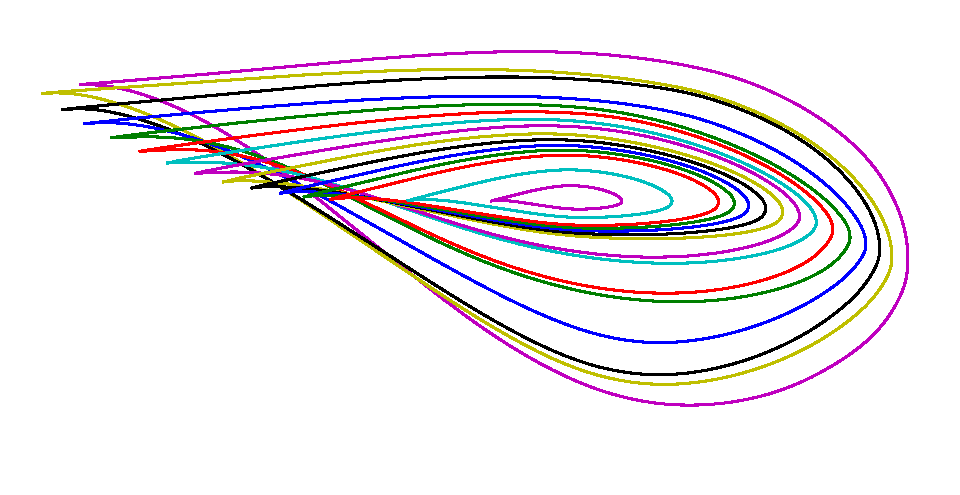
\includegraphics[width=0.49\linewidth]{airfoils-note}
    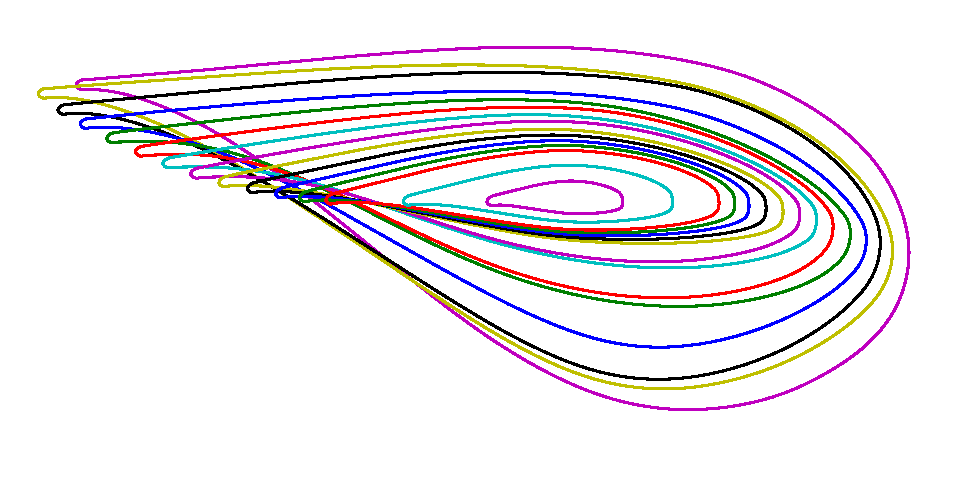
\includegraphics[width=0.49\linewidth]{airfoils-te}
    \captionof{figure}{Artificial rounding of each airfoil allows a more efficient mesh.}
  \end{center}
  \begin{center}
    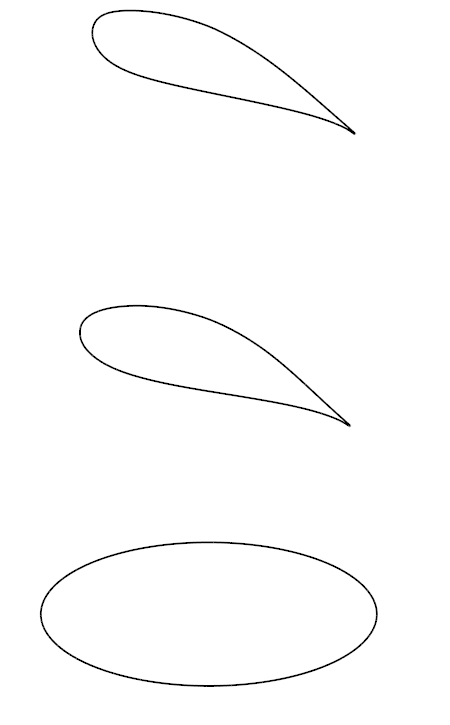
\includegraphics[width=0.23\textwidth]{figs/length-none}
    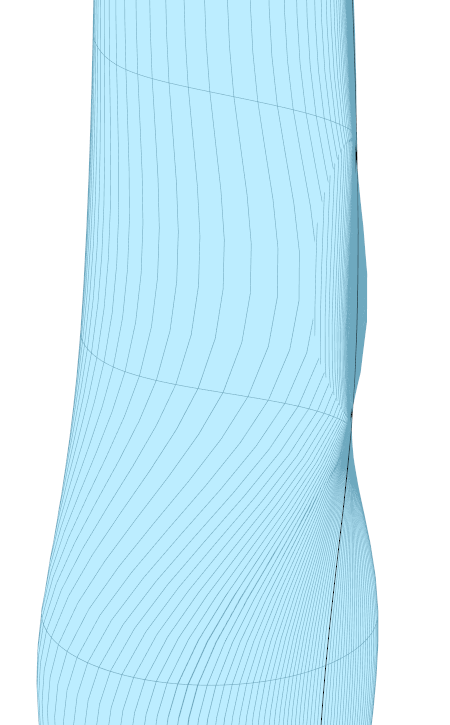
\includegraphics[width=0.23\textwidth]{figs/length-none-surf}
    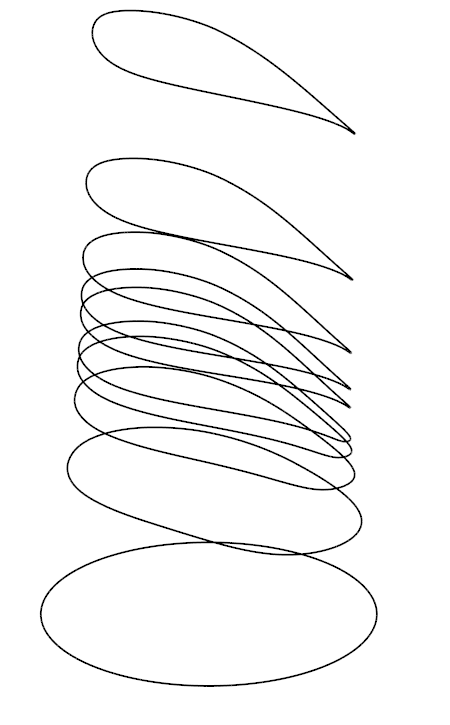
\includegraphics[width=0.23\textwidth]{figs/length-joined}
    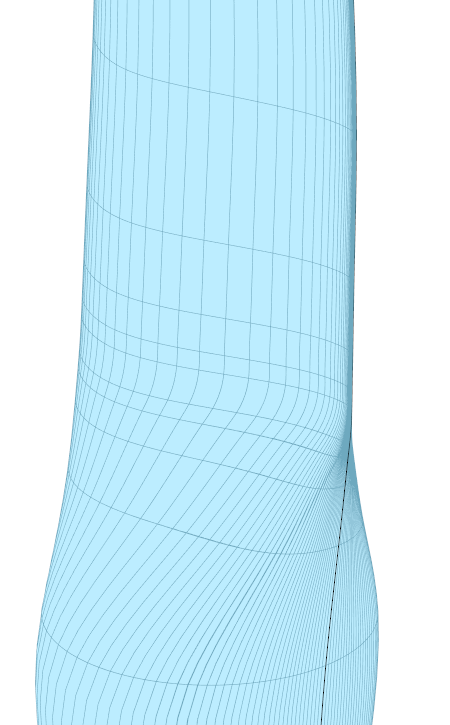
\includegraphics[width=0.23\textwidth]{figs/length-joined-surf}
    \captionof{figure}{Two-step interpolation routine with low and high order avoids a self-intersecting mesh.}
  \end{center}
}

\headerbox{Conclusion}{name=conclusion,column=0,below=methods}{
  The mesh generator has been used in practice for the NREL 5MW blade in various configurations (no
  tip, cut-off tip, rounded tip), as well as a for other verification blades.  It is easily
  controlled with parameters for geometry, resolution, load balancing and output format, such as
  OpenFOAM.  It can also produce other meshes with the same topology.
}

\headerbox{References}{name=references,column=0,below=conclusion}{
  \smaller
  \renewcommand{\section}[2]{\vskip 0.0em}
  \bibliographystyle{unsrt}
  \bibliography{common/references}
}

\headerbox{Acknowledgements}{name=acknowledgements,column=0,below=references, above=bottom}{
  \smaller
  The authors acknowledge the financial support from the Norwegian Research Council and the
  industrial partners of the FSI-WT (216465/E20) (\url{fsi-wt.no}) and NOWITECH: Norwegian Research
  Centre for Offshore Wind Technology (\url{nowitech.no}) projects.
}

\headerbox{Two-dimensional mesh generation}{name=results1,span=2,column=1,row=0}{
  We envelop each airfoil in a circle and use transfinite interpolation\cite{Gordon1973ccc} (TFI) to
  generate the intervening ``O-mesh''.  It is then split in eight patches and extended as necessary.
  \begin{center}
    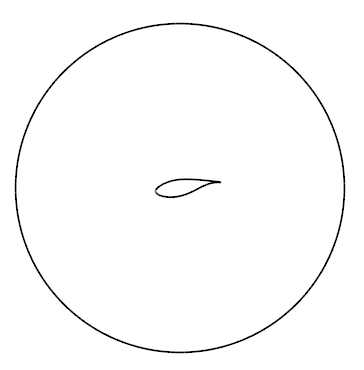
\includegraphics[width=0.2\linewidth]{tfi-1}
    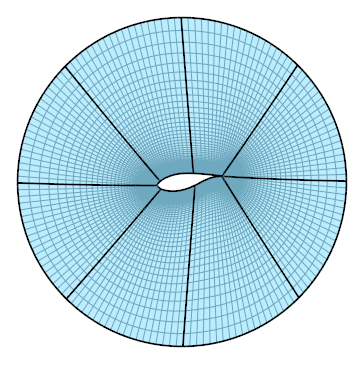
\includegraphics[width=0.2\linewidth]{tfi-2}
    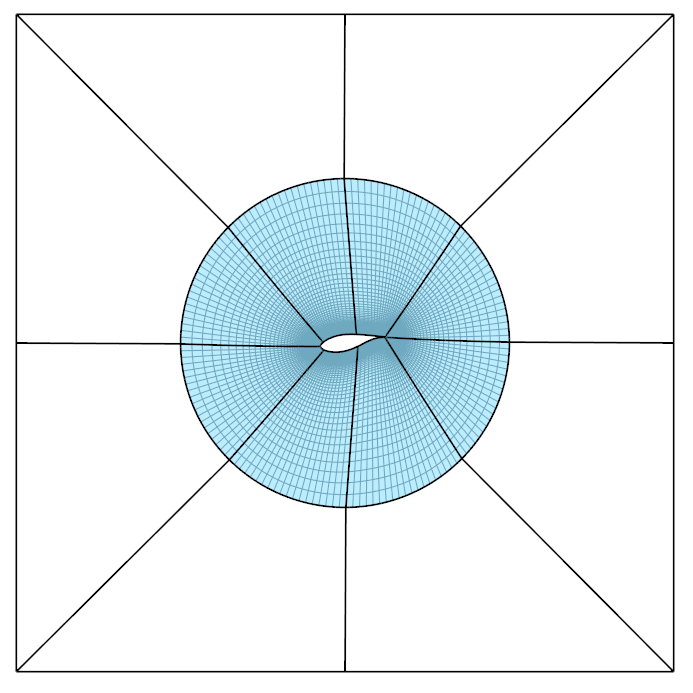
\includegraphics[width=0.2\linewidth]{tfi-3}
    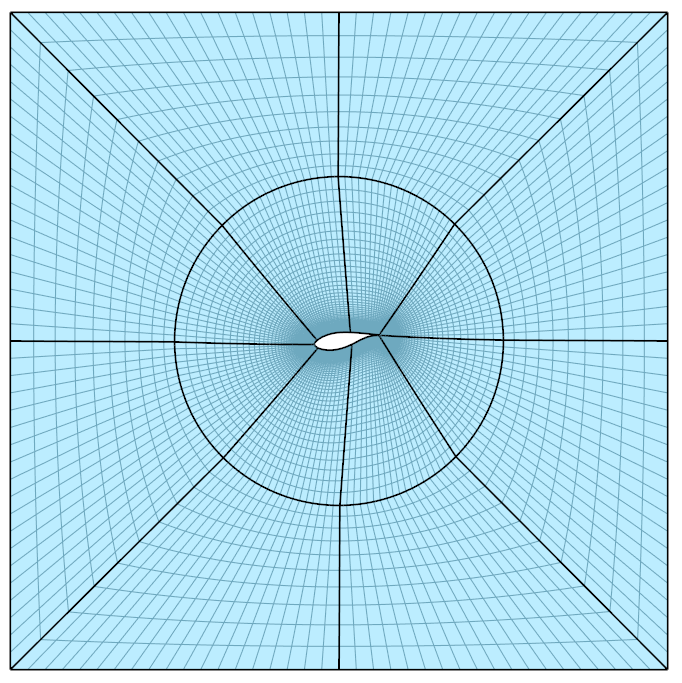
\includegraphics[width=0.2\linewidth]{tfi-4}
  \end{center}
  \begin{itemize}
    \item The mesh generated is highly sensitive to parametrization (not just geometry).
      This is solved using a parameter-normalization technique.
    \item TFI cannot guarantee orthogonal meshlines close to the body, which is necessary for our
      applications.  This is solved by ``growing'' the mesh layer-by-layer, using at each step a
      weighted average between regular TFI and orthogonal projection.
    \item Gridlines might intersect in rare cases (highly concave domains.)  This is solved by
      applying a Laplacian smoothing at each layer.
  \end{itemize}
  \begin{center}
    \raisebox{-0.5\height}{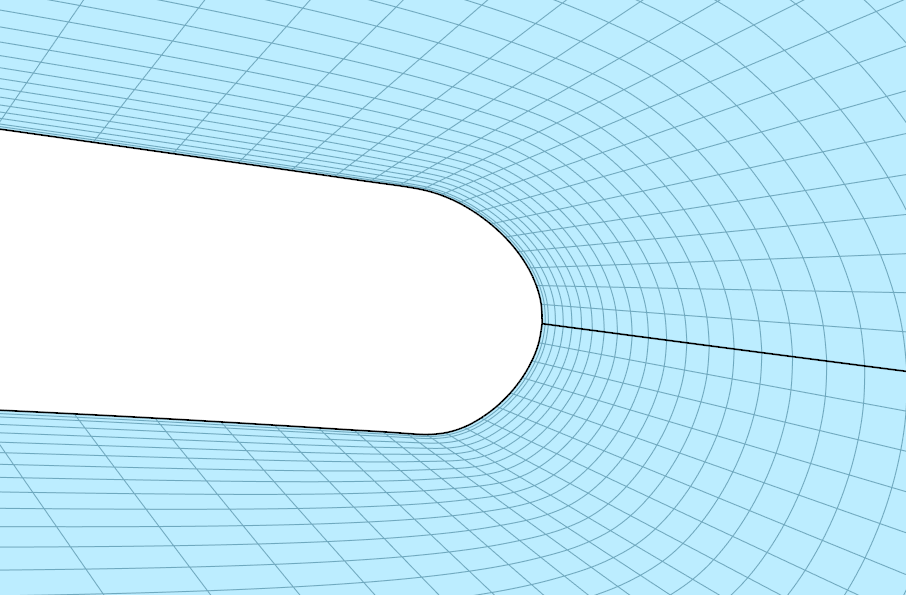
\includegraphics[width=0.2\linewidth]{nonorthogonal}}
    \raisebox{-0.5\height}{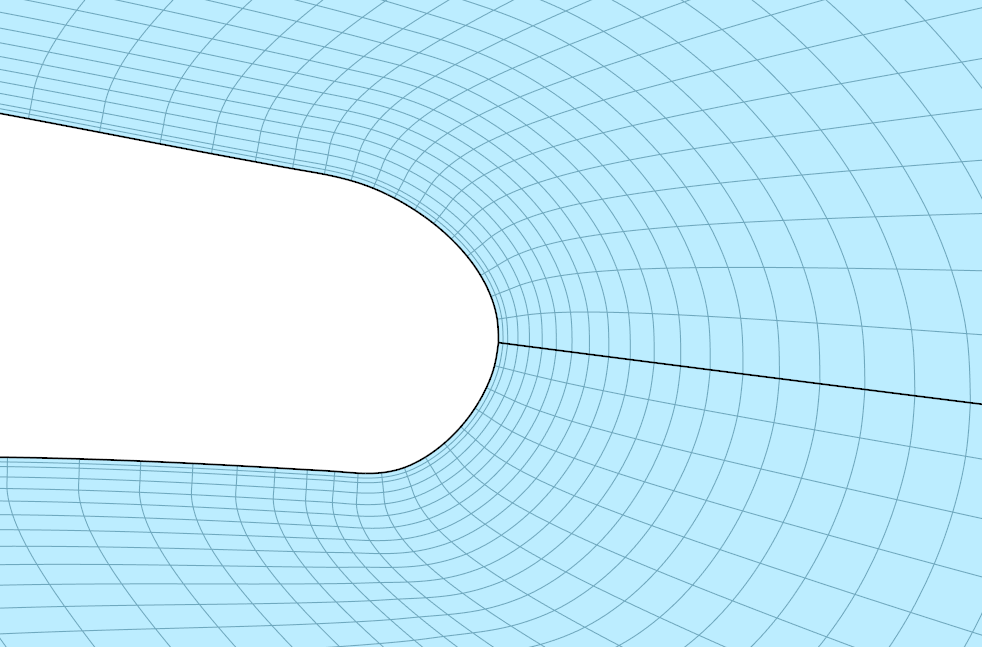
\includegraphics[width=0.2\linewidth]{orthogonal}}
    \raisebox{-0.5\height}{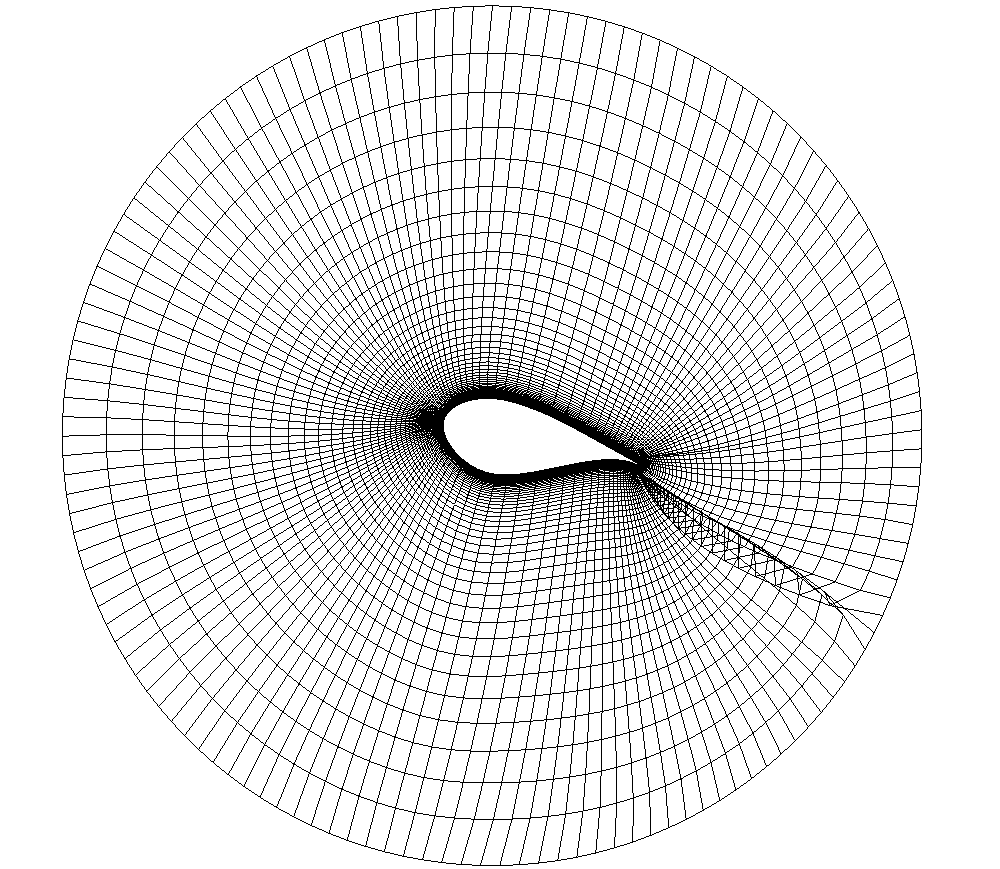
\includegraphics[width=0.2\linewidth]{section12}}
    \raisebox{-0.5\height}{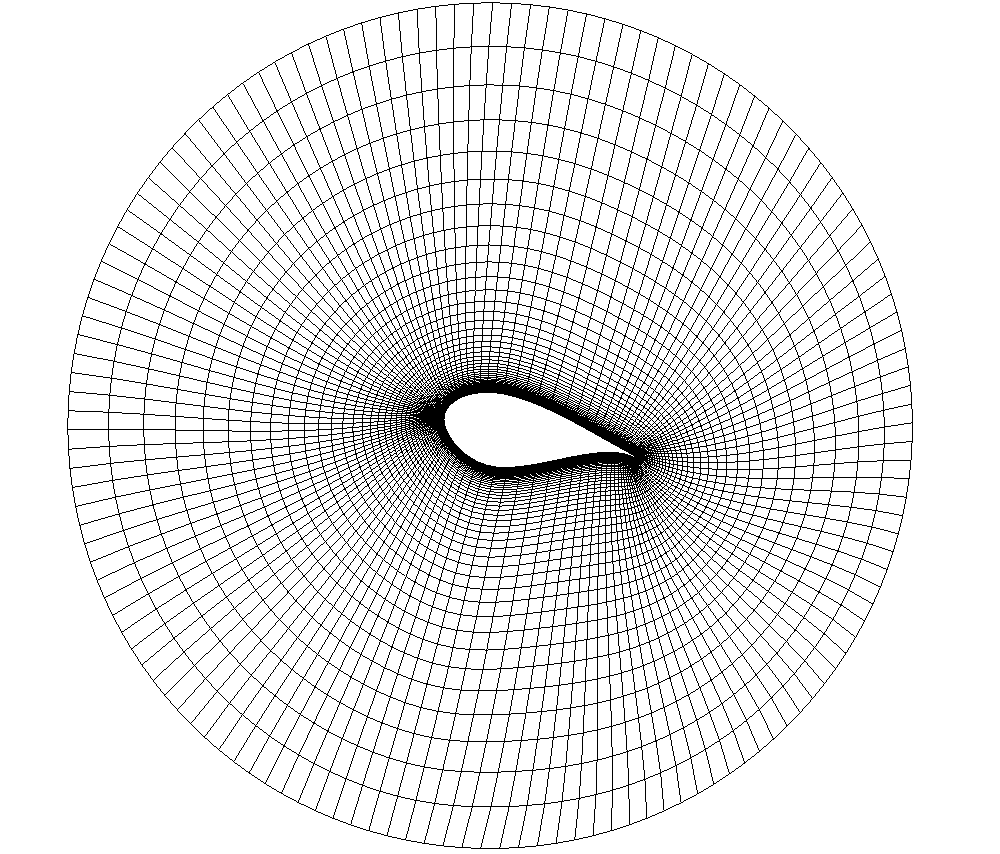
\includegraphics[width=0.2\linewidth]{section12_smooth}}
    \captionof{figure}{Orthogonalization (left) and smoothing (right).}
  \end{center}
}

\headerbox{Tip closure}{name=results2,span=2,column=1,below=results1}{
  To construct the tip, we raise the midline of the final airfoil some suitable distance (here,
  about $\SI{20}{cm}$).  Then, interpolation between the opposite sides of the airfoil and the
  raised midline generates a family of curves that produces a parametrization of the tip with two
  singularities.  This surface is then sectioned into twelve patches without singularities.
  \begin{center}
    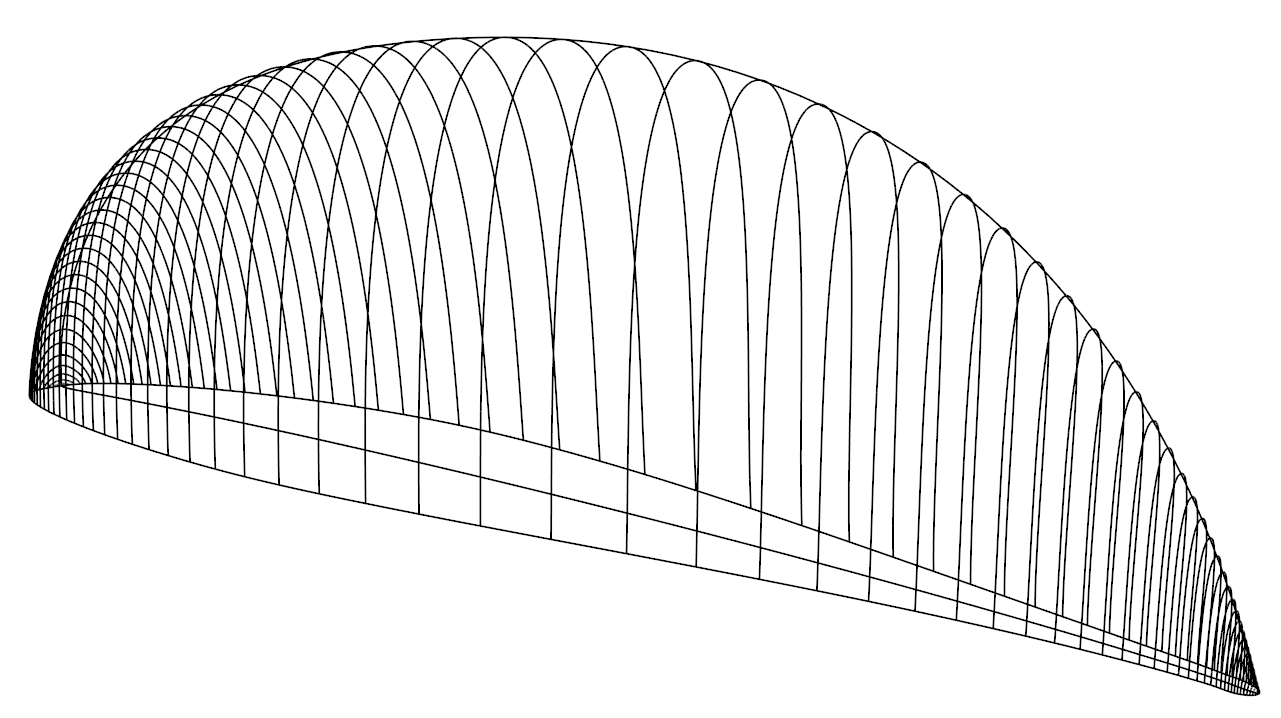
\includegraphics[width=0.3\linewidth]{wingtip-skeleton}
    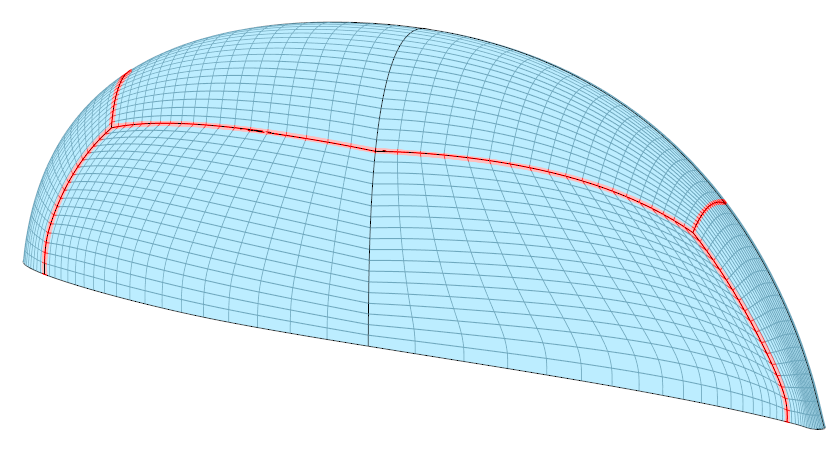
\includegraphics[width=0.3\linewidth]{wingtip-full}
  \end{center}
  The surrounding mesh can then be generated using a relatively straightforward volumetric
  generalization of the described TFI algorithm.
  \begin{center}
    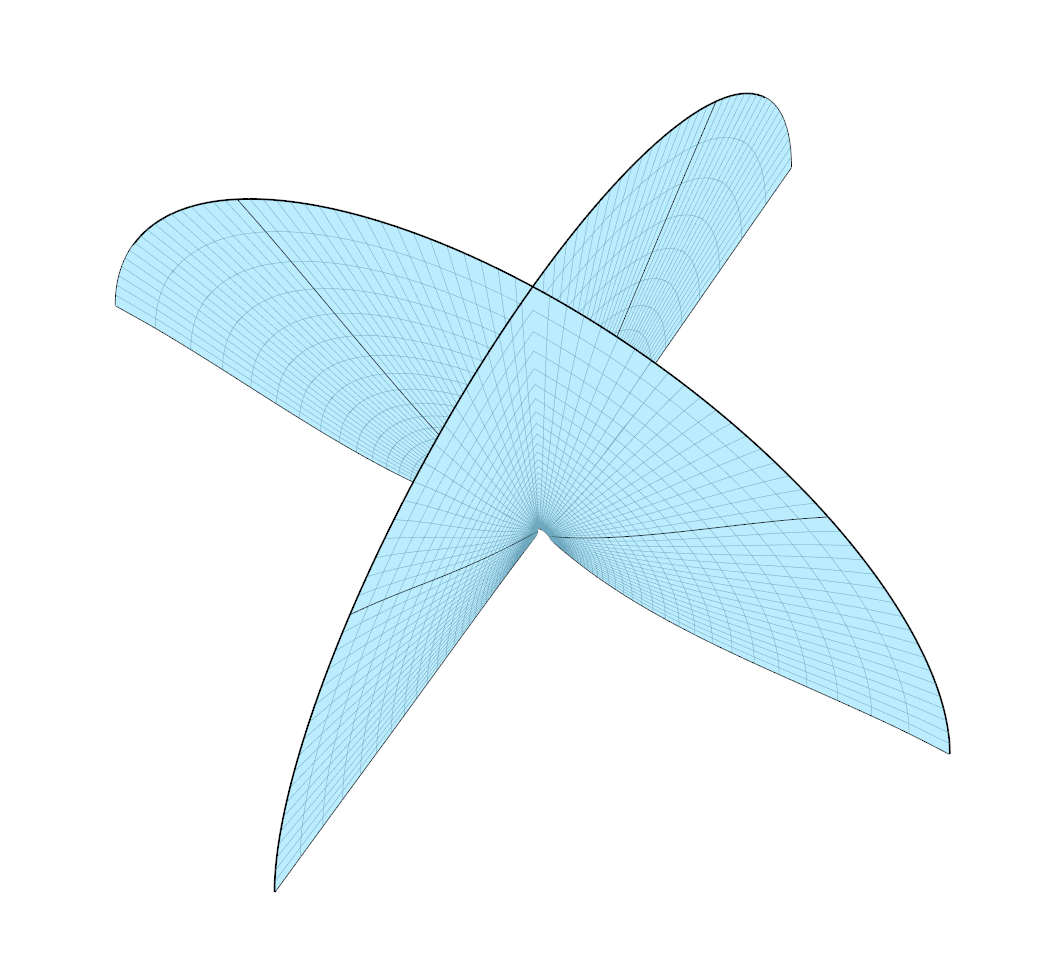
\includegraphics[width=0.25\linewidth]{wingtip-first}
    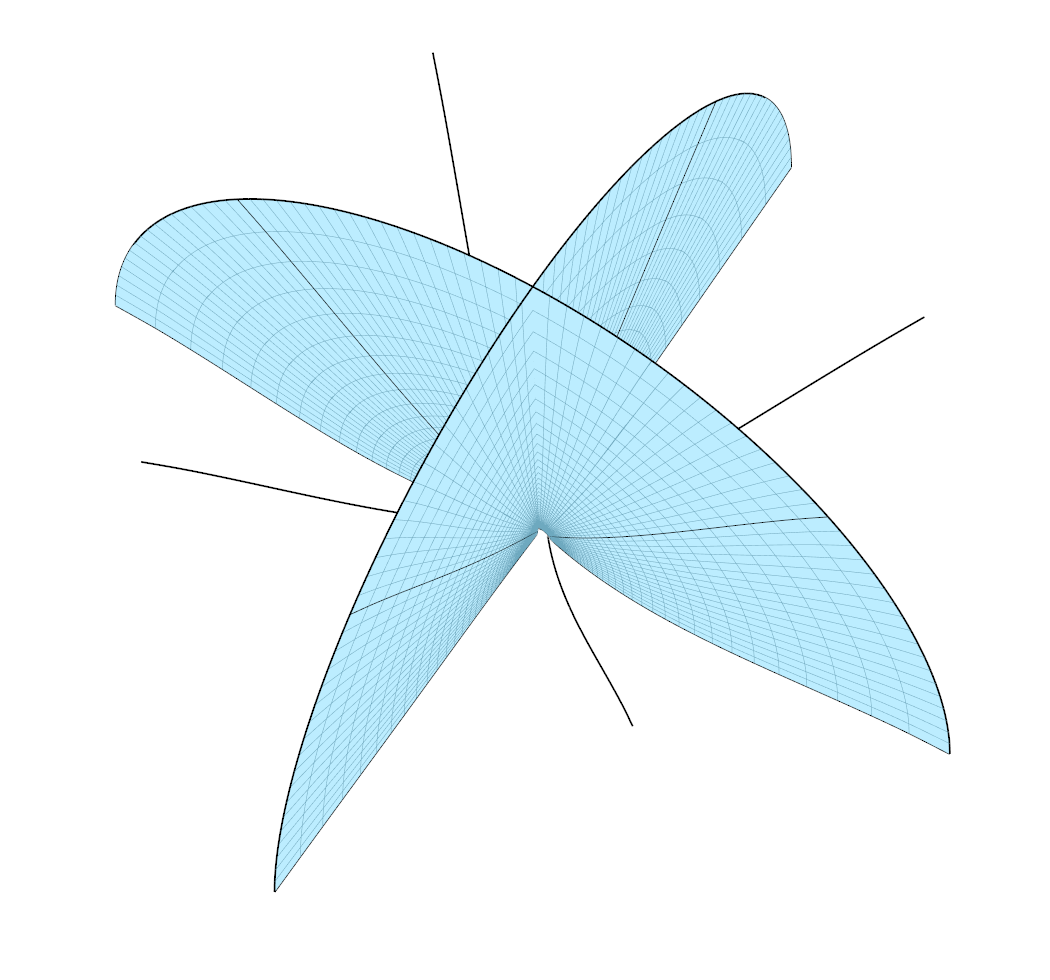
\includegraphics[width=0.25\linewidth]{wingtip-centers}
    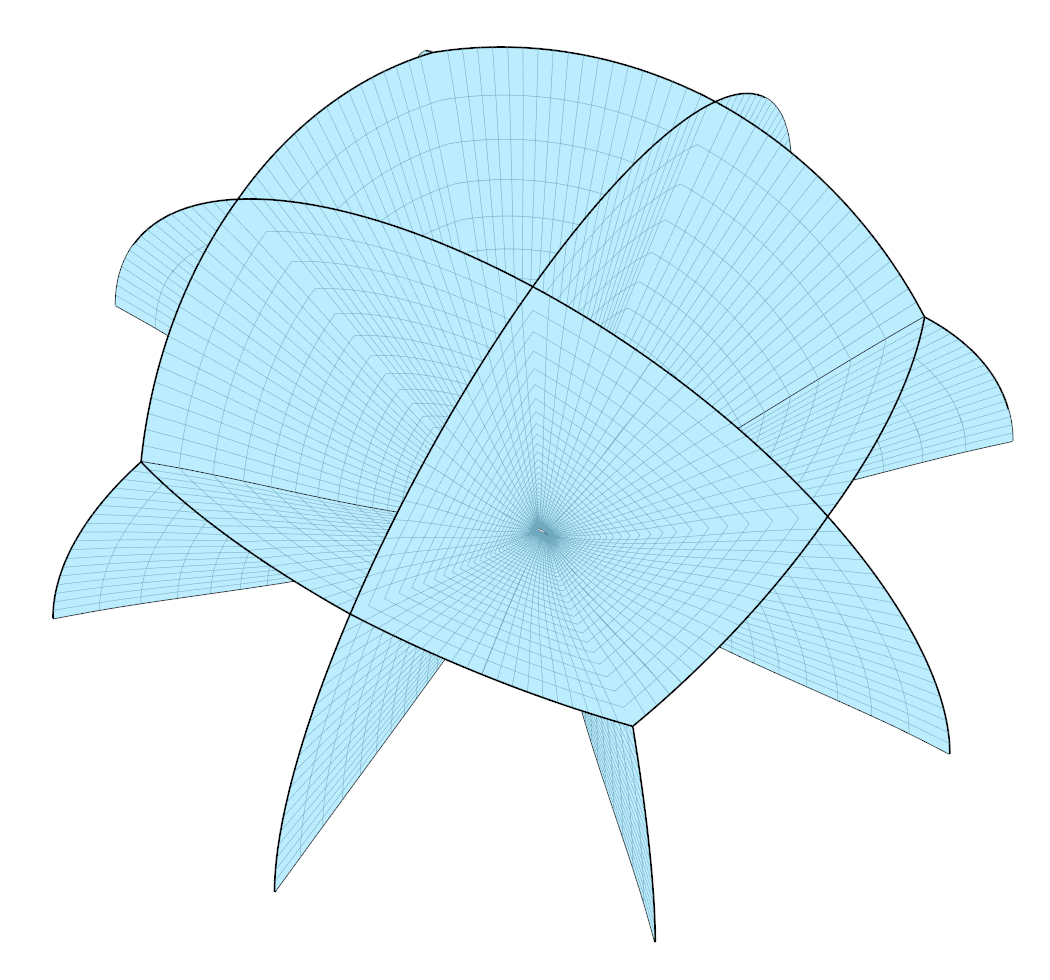
\includegraphics[width=0.25\linewidth]{wingtip-flower}
  \end{center}
}

\headerbox{Block structure}{name=results3,span=2,column=1,below=results2,above=bottom}{
  The final block structure of the mesh consists of eight sectors (four on the tip), and an
  arbitrary number of decompositions in the radial and lengthwise directions.
  \begin{center}
    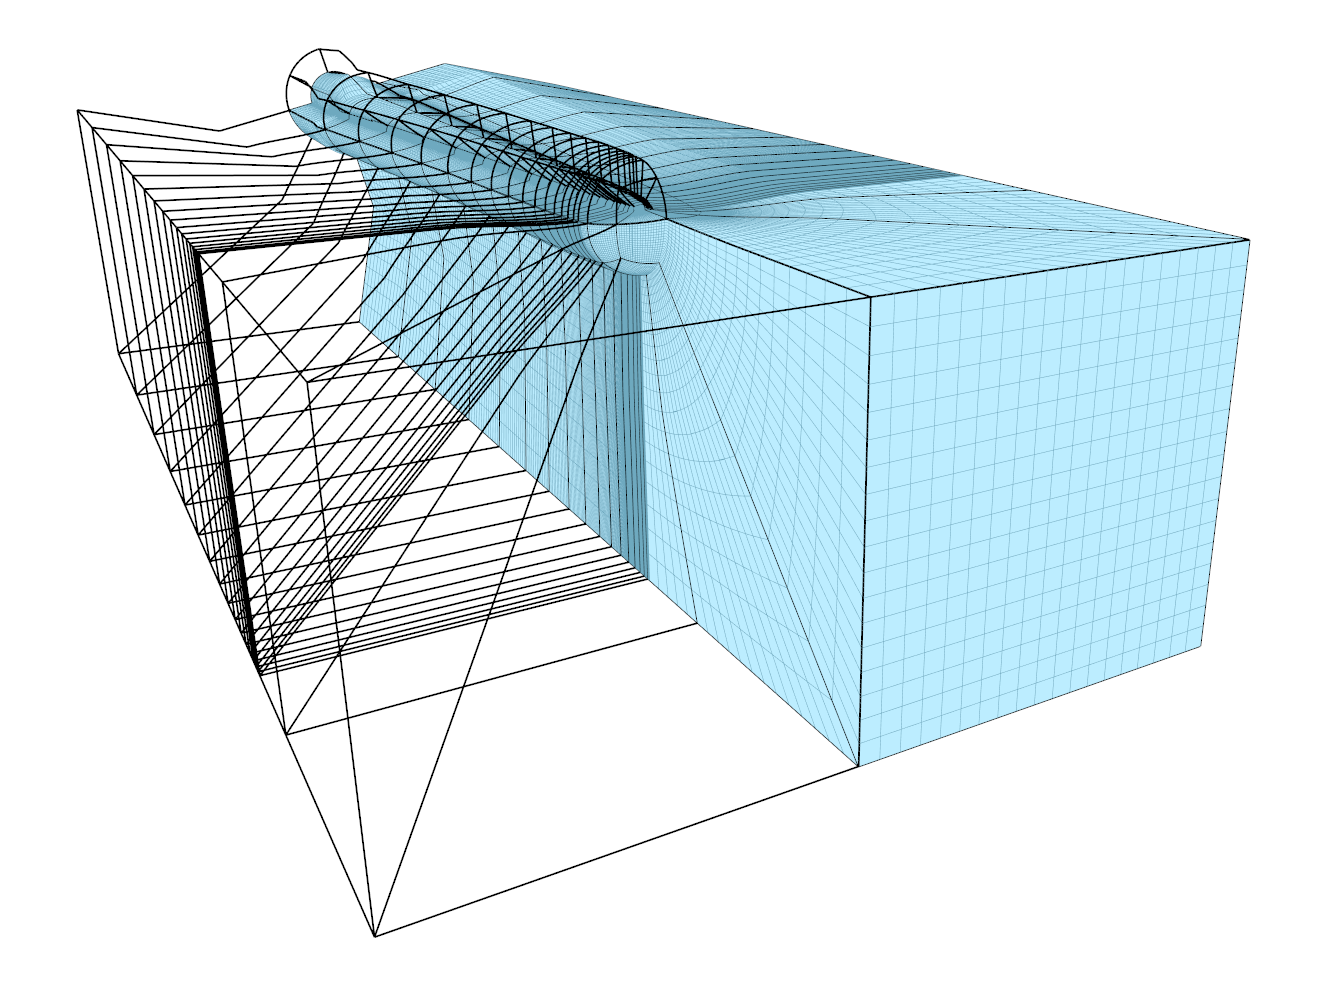
\includegraphics[width=0.32\linewidth]{block-1}
    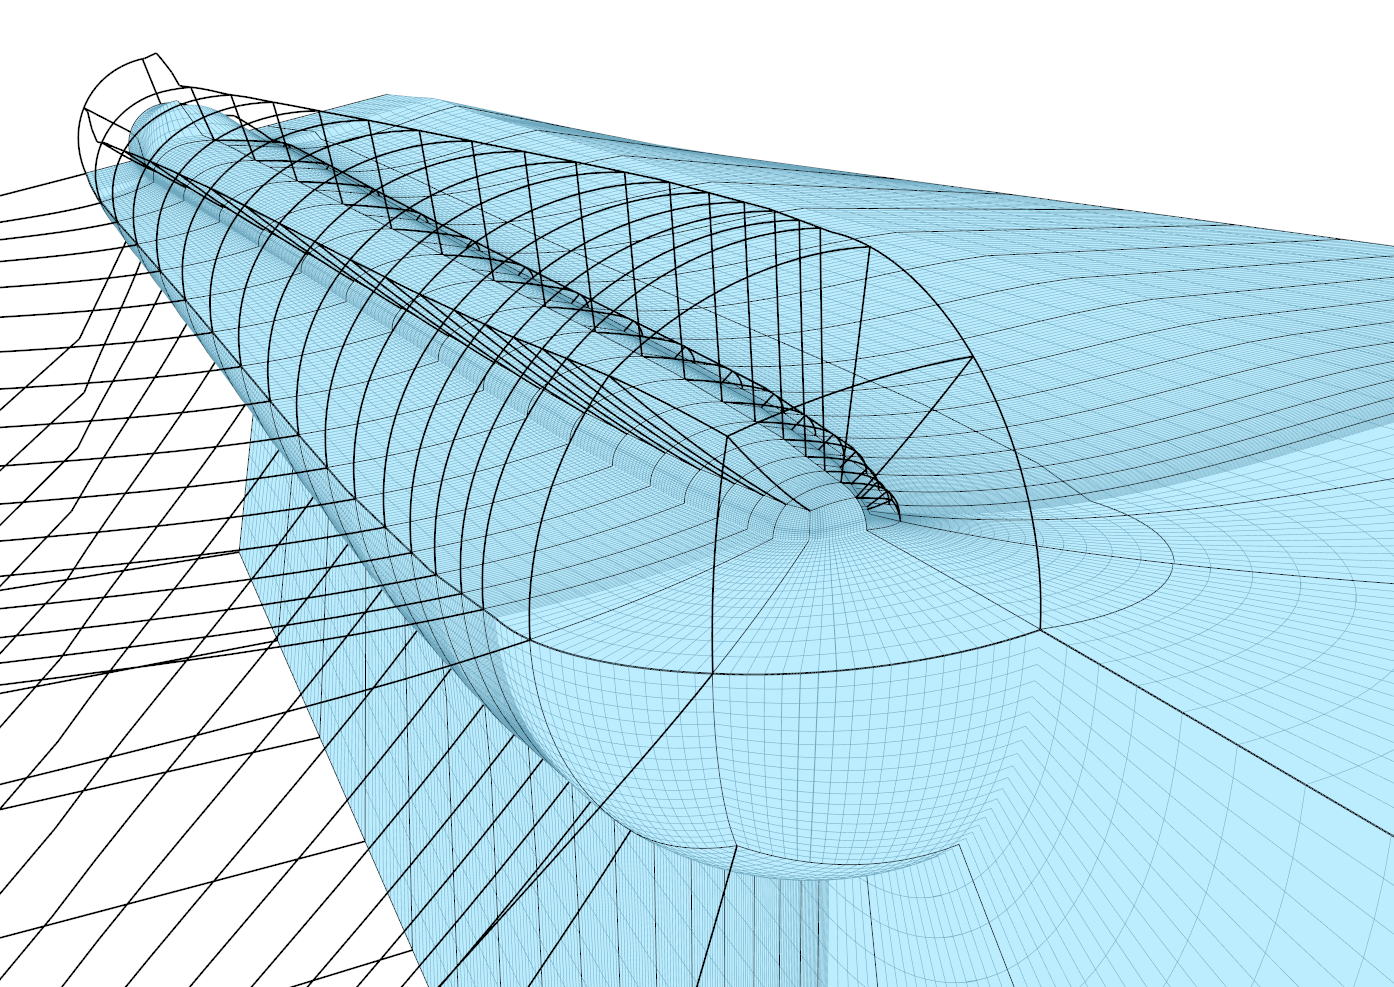
\includegraphics[width=0.32\linewidth]{block-2}
    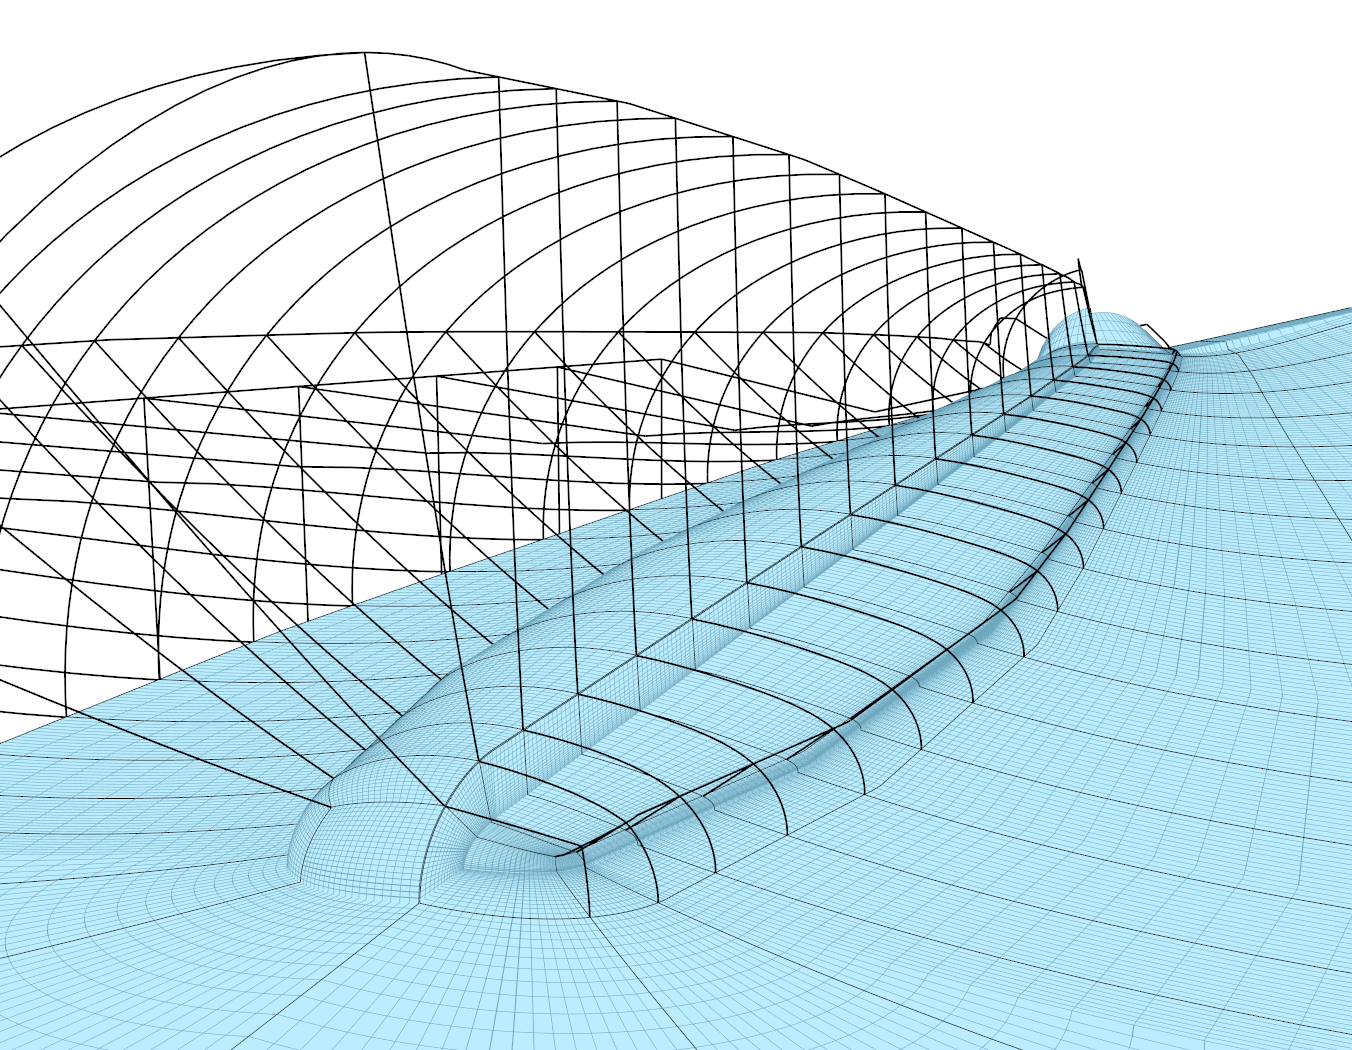
\includegraphics[width=0.32\linewidth]{block-3}
  \end{center}
}

\end{poster}

\end{document}
